\subsection{Consuntivo fase di progettazione}
Il bilancio della fase di progettazione è positivo. Il gruppo ha impiegato meno ore di quelle preventivate inzialmente ma sono stati riscontrati diversi problemi.\\
È stato cruciale fare un'analisi critica della fase precedente e dei rischi che ne possono derivare: sono stati riscontrati rischi che hanno influito nella ripianificazione della fase di progettazione.
Il team ha concordato ad unanimità di ruotare i ruoli in modo solo parziale e lasciare la progettazione architetturale e lo sviluppo relativo al \glo{PoC} a membri con un'esperienza maggiore nelle relative tecnologie conivolte.
Per l'analisi dei rischi riscontrati si rimanda alla \hypersetup{
    linkcolor=blue
} \hyperlink{Tabellaoccorrenzarischi}{tabella dell'occorrenza dei rischi} 
\hypersetup{
    linkcolor=black
}
in appendice.
Gli incrementi sviluppati in tale fase sono:\\
\begin{itemize}
	\item l'incremento 0. 
\end{itemize}
Il costo di tale incremento essendo unico è essenzialmente il costo orario del progettista e del programmatore, più qualche ora di test d'integrita manuale, maggiori dettagli relativi a questo incremento(0) si trovano in appendice, nella 
\hypersetup{
    linkcolor=blue
}
\hyperlink{TabellaIncrementi}{tabella degli incrementi}.\hypersetup{
    linkcolor=black
}
La seguente tabella illustra la differenza oraria ed economica rilevata a posteriori.
{
\rowcolors{2}{\evenRowColor}{\oddRowColor}
\renewcommand{\arraystretch}{2}
\begin{longtable}[h]{ C{2.5cm} C{2cm} C{1.8cm} C{2.2cm} C{1.5cm} C{2.3cm}}
\caption{Tabella del costo complessivo per ruolo}\\
\rowcolor{\primaryColor}

\textcolor{\secondaryColor}{\textbf{Ruolo}} & 
\textcolor{\secondaryColor}{\textbf{Ore preventivate}} & 
\textcolor{\secondaryColor}{\textbf{Variazione oraria}} & 
\textcolor{\secondaryColor}{\textbf{Costo preventivato (in \euro{})}} & 
\textcolor{\secondaryColor}{\textbf{Costo effettivo (in \euro{})}} & 
\textcolor{\secondaryColor}{\textbf{Variazione di costo (in \euro{})}}\\	
	
Responsabile    &  19 & 0 & 630 & 570 &  0 \\
Amministratore  &  20 & 0 & 400 & 400 & 0 \\
Analista        & 24 & +16 & 600 & 1000 & +400 \\
Progettista     &  49 & -9 & 1078 & 880 & -198 \\
Programmatore   &   58 & -12 & 870 &  690 & -180 \\
Verificatore    &  59 &  -10 & 885 & 735 & -150 \\
\textbf{Totale} & 231 & 15 & 4463 & 4335 & -128 \\	
\end{longtable}
}

 \begin{figure}[h!]
	\caption{Istogramma di ridistribuzione oraria e delle responsabilità relativo alla fase di progettazione}
    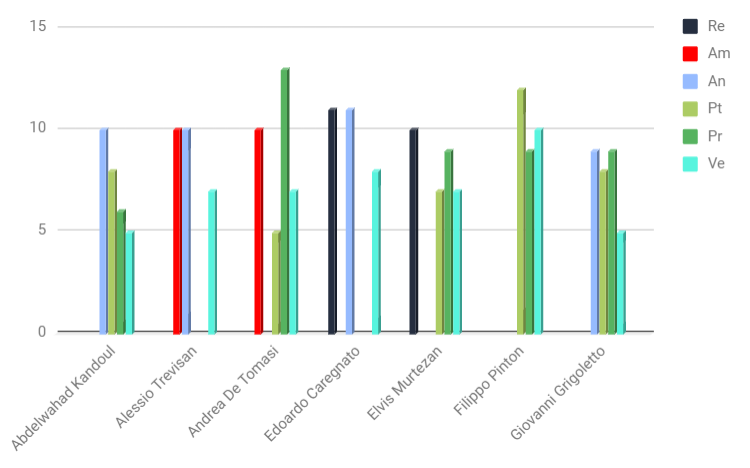
\includegraphics[width=1\textwidth]{./src/Preventivo/src/img/istoConsuntivoProgettazioneRuoli.png}  
\end{figure} 


\subsubsection{Conclusioni}
Come riportato dalla tabella, il bilancio risulta essere positivo per i seguenti motivi:
\begin{itemize}
	\item \textbf{Responsabile}: {essendo il team abbastanza coeso la maggior parte del tempo è stata dedicato al PdP;}
	\item \textbf{Amministratore}: {la collaborazione tra membri del team in questo ruolo è risultata soddisfaciente;}
	\item \textbf{Analista}: {dopo l'aggiudicazione del capitolato il team si è reso conto che la documentazione presente nell'AdR presentava diverse lacune, ciò ha portato a un incremento orario per tale ruolo;}
	\item \textbf{Progettista}: {grazie all'esperienza dei membri e alla chiarezza dei requisiti si è riuscito a mitigare il numero di ore neccessarie a progettare il PoC, ammortizzando il costo orario dell'analista;}
	\item \textbf{Programmatore}: {grazie all'esperienza dei membri e alla chiarezza dei requisiti si è riuscito a mitigare il numero di ore neccessarie allo sviluppo del PoC, ammortizzando il costo orario dell'analista;}
	\item \textbf{Verificatore}: {avendo più esperienza con le tecnologie richieste(alla documentazione in particolare), il numero di ore è inferiore a quelle preventivate.}
\end{itemize}
\subsubsection{Ragionamento sugli scostamenti futuri}
L'esperienza e la coesione maturata saranno cruciali nel cercare di mitigare il numero di ore richieste, visti gli scostamenti orari (in particolare dell'analista) rispetto al preventivo iniziale, che hanno portato ad una riduzione oraria complessiva di ciascun membro.
Visti i problemi riscontrati nel bilancio della fase di progettazione, il costo totale del preventivo a finire rimarrà invariato, per mitigare eventuali rischi (come quelli riscontrati in tale fase) o investirli nell'implementazione di requisiti desiderabili o facoltativi.



La seguente tabella rappresenta la ridistribuzione oraria dei ruoli per ogni componente del gruppo:
\rowcolors{2}{\evenRowColor}{\oddRowColor}
\renewcommand{\arraystretch}{2}
\begin{longtable}[h!] { C{3.5cm} C{1cm} C{1cm} C{1cm} C{1cm} C{1cm} C{1cm} C{2cm}}
\caption{Ridistribuzione oraria preventivo a finire}\\
\rowcolor{\primaryColor}

\textcolor{\secondaryColor}{\textbf{Membro del gruppo}} & 
\textcolor{\secondaryColor}{\textbf{RE}} & 
\textcolor{\secondaryColor}{\textbf{AM}} & 
\textcolor{\secondaryColor}{\textbf{AN}} & 
\textcolor{\secondaryColor}{\textbf{PT}} & 
\textcolor{\secondaryColor}{\textbf{PR}} & 
\textcolor{\secondaryColor}{\textbf{VE}} & 
\textcolor{\secondaryColor}{\textbf{Ore complessive}}\\	
\endhead
        
\AW{}                     & -  & 5 & 10 & 30 & 25 & 32 & 102 \\
\AT{}                     & 11 & 10 & 15& 15 & 22 & 28 & 101\\
\AD{}                     & 10 & 10 & 0 & 12 & 38 & 32 & 102 \\
\EC{}                     & 11 & 10 & 11& 13 & 23 & 32 & 100 \\
\EM{}                     & 10 & 8 & 0 & 17 & 38 & 30 & 103 \\
\FP{}                     & 10 & 8 & 0 & 23 & 34 & 27 & 102 \\
\GG{}                     & -  & 8 & 9 & 23 & 35 & 27 & 102 \\
\textbf{Ore totali ruolo(variazione)} & 52 & 59 & 45(+16) & 133(-9) & 215(-12) & 208(-10) & 712(-15) \\


\end{longtable}

\clearpage		
\begin{figure}[h!]
	\centering
	\caption{Istogramma di ridistribuzione oraria del preventivo a finire}
    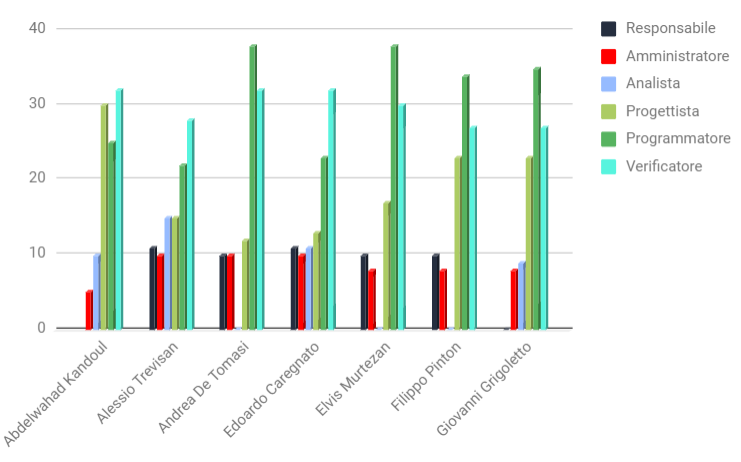
\includegraphics[width=1\textwidth]{./src/Preventivo/src/img/IstoPreventivoaFinireProj.png}  
\end{figure} 

